%----------------------------------------------------------------------------------------
%	PACKAGES AND THEMES
%----------------------------------------------------------------------------------------
\documentclass[aspectratio=169,xcolor=dvipsnames]{beamer}
\usetheme{Simple}

\usepackage{hyperref}
\usepackage{graphicx} % Allows including images
\usepackage{booktabs} % Allows the use of \toprule, \midrule and \bottomrule in tables
\usepackage{tikz}
\usepackage{caption}
\usetikzlibrary{positioning}
\usepackage{amsmath}


%----------------------------------------------------------------------------------------
% Title Slide
%----------------------------------------------------------------------------------------

% The title
\title[short title]{The Optimization of Flight Routes: Enhancing Connectivity and Reducing Cost}
\subtitle{Leveraging Optimization Models for Profitability!}

\author[] {Ian Wald}
\institute[] % Your institution may be shorthand to save space
{
    % Your institution for the title page
    Institute for Computing in Research \\
    Santa Fe, New Mexico
    \vskip 3pt
}
\date{August 2, 2024} % Date, can be changed to a custom date


%----------------------------------------------------------------------------------------
% Title Slide
%----------------------------------------------------------------------------------------

\begin{document}

\begin{frame}
    % Print the title page as the first slide
    \titlepage
\end{frame}

%------------------------------------------------
\section{Context}
%------------------------------------------------

\begin{frame}{Context}
\centering 
    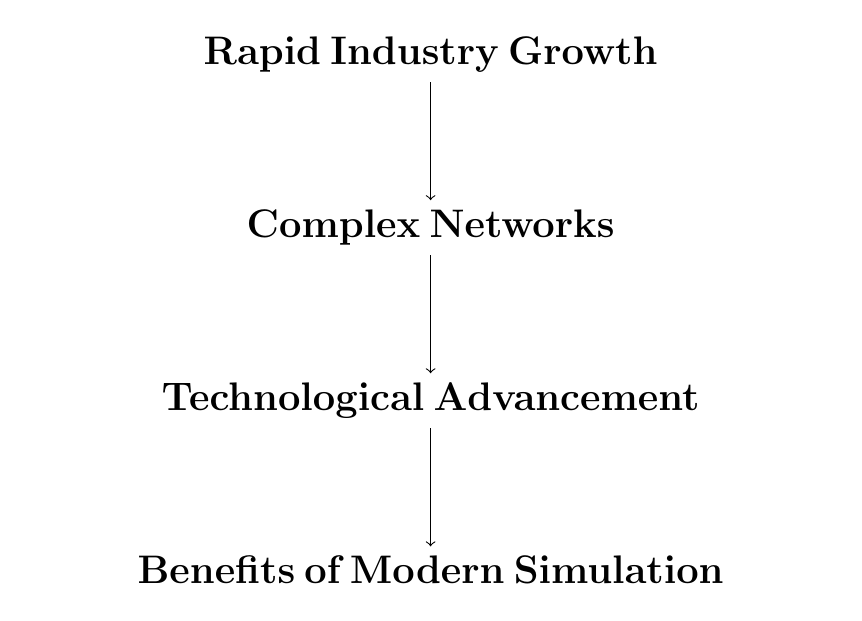
\begin{tikzpicture}[node distance=1.5cm, auto]
        \node (A) [text width=10cm, align=center] {
            \large
            \Large\textbf{Rapid Industry Growth}
        };

        \node (B) [below=of A, text width=10cm, align=center] {
            \Large\textbf{Complex Networks}
        };

        \node (C) [below=of B, text width=10cm, align=center] {
            \Large\textbf{Technological Advancement}
        };

        \node (D) [below=of C, text width=10cm, align=center] {
            \Large\textbf{Benefits of Modern Simulation}
        };
        
        % Drawing lines between the points
        \draw[->] (A.south) -- (B.north);
        \draw[->] (B.south) -- (C.north);
        \draw[->] (C.south) -- (D.north);
    \end{tikzpicture}   
\end{frame}

%------------------------------------------------
\section{Research Question}
%------------------------------------------------
\begin{frame}{Research Question}
        \begin{center}
        \LARGE
        \textbf{What variables can airlines manipulate to optimize flight routes across the continental United States to enhance efficiency and maximize profitability?}
    \end{center}  
\end{frame}

%---------------------------------------------------------

\begin{frame}{Flight Route Optimization vs. Standard Optimization}
    \begin{minipage}{0.45\textwidth}
        \centering
        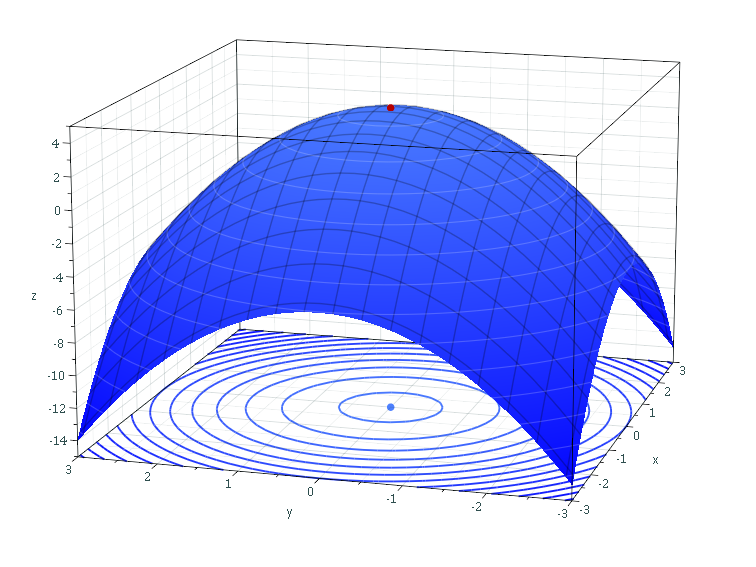
\includegraphics[width=\textwidth]{images/MaximumParaboloid.png}
        \captionof{figure}{Example of a Standard Optimized Plot}
    \end{minipage}
    \hfill
    \begin{minipage}{0.5\textwidth}
        \begin{itemize}
            \item \textbf{Discrete Decision Making:}
            \begin{itemize}
                \item All-or-Nothing Routes
                \item Incremental Adjustments
            \end{itemize}
            
            \item \textbf{Strict Operational Constraints:}
            \begin{itemize}
                \item Fixed vs Dynamic Variables
                \item Levels of Flexibility on Constraints
            \end{itemize}
            
            \item \textbf{Data Integration:}
            \begin{itemize}
                \item Simulation vs Functions
                \item Balanced vs Feasible Solutions
            \end{itemize}
        \end{itemize}
    \end{minipage}
\end{frame}

%------------------------------------------------
\section{Strategy}
%------------------------------------------------

\begin{frame}{Strategy of the Three Algorithms}
    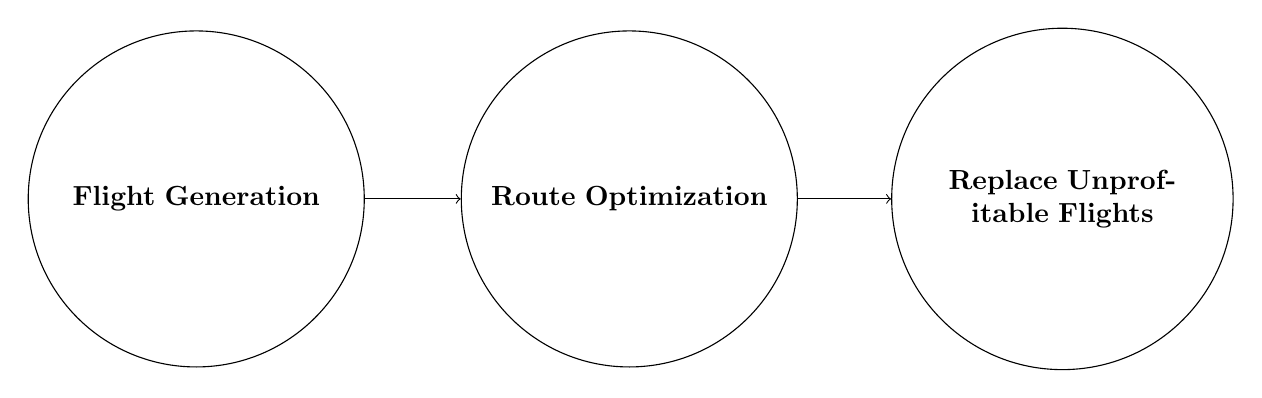
\begin{tikzpicture}[node distance=3cm, auto]
        % Node definitions
        \node (A) [draw, shape=circle, minimum size=3cm, align=center, text width=4cm] {
            \textbf{Flight Generation}
        };

        \node (B) [draw, shape=circle, minimum size=3cm, align=center, text width=4cm, right of=A, xshift=2.5cm] {
            \textbf{Route Optimization}
        };

        \node (C) [draw, shape=circle, minimum size=3cm, align=center, text width=4cm, right of=B, xshift=2.5cm] {
            \textbf{Replace Unprofitable Flights}
        };
        
        % Connecting lines
        \draw[->] (A) -- (B);
        \draw[->] (B) -- (C);
    \end{tikzpicture}
\end{frame}

%------------------------------------------------
\section{Flight Generator}
%------------------------------------------------

\begin{frame}{Flight Generation}
    \begin{minipage}{0.45\textwidth}
        \centering
        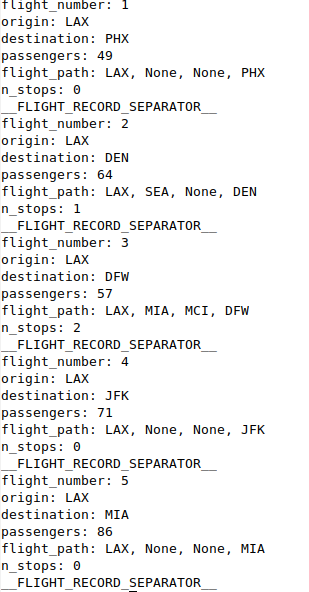
\includegraphics[width=\textwidth]{images/flight_output.png}
    \end{minipage}
    \hfill
    \begin{minipage}{0.5\textwidth}
        \vspace{-5.5cm} 
        \textbf{Overview:}
        \begin{itemize}
            \item Generate all possible flights from predefined airports
            \item Base File Pior for Modification
        \end{itemize}
        \vspace{0.5cm}
        \textbf{Details:}
        \begin{itemize}
            \item Produces flights from one airport (origin) to all other listed airports
            \item Random number of stops and amount of passengers
            \item IATA codes with an associated latitude and longitude coordinate.
        \end{itemize}
        \captionof{figure}{Output within \texttt{generated\_flights\_new.txt}}
    \end{minipage}
\end{frame}

%------------------------------------------------
\section{Haversine Formula}
%------------------------------------------------

\begin{frame}{Haversine Formula}
    \begin{minipage}[t]{0.5\textwidth}
        \vspace{-3cm} 
        \textbf{Description:} \\
        \vspace{0.1cm} % Adjust vertical spacing if necessary
        \[
        a = \sin^2\left(\frac{\Delta \phi}{2}\right) + \cos(\phi_1) \cdot \cos(\phi_2) \cdot \sin^2\left(\frac{\Delta \lambda}{2}\right)
        \]
        \[
        c = 2 \cdot \text{atan2}\left(\sqrt{a}, \sqrt{1-a}\right)
        \]
        \[
        d = R \cdot c
        \]
        where \( \phi_1 \) and \( \phi_2 \) are the latitudes, \( \Delta \phi \) and \( \Delta \lambda \) are the differences in latitudes and longitudes, and \( R \) is the Earth's radius.
    \end{minipage}
    \hfill
    \begin{minipage}{0.45\textwidth}
        \centering
        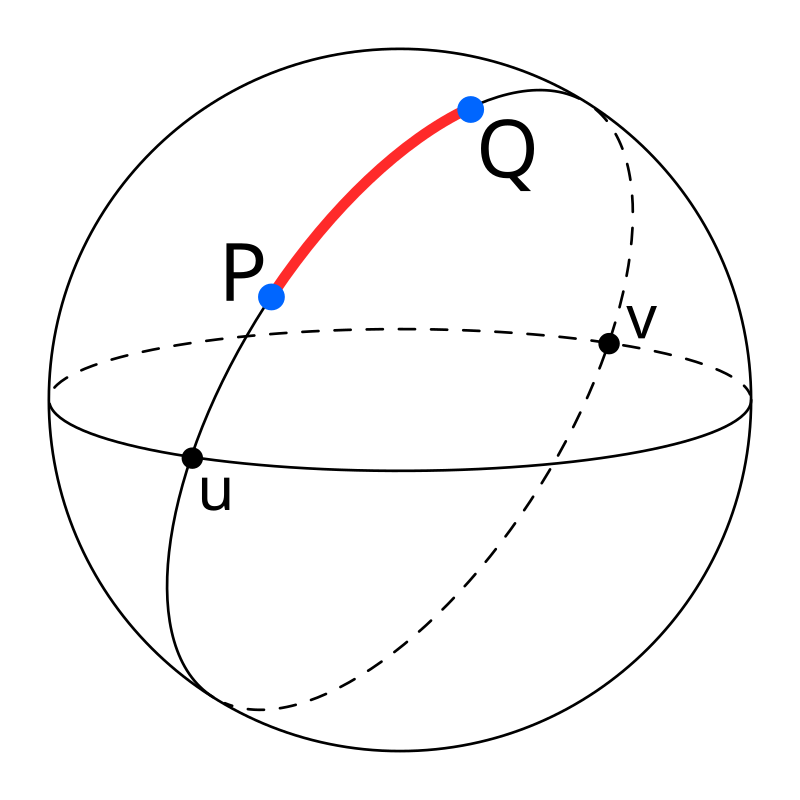
\includegraphics[width=\textwidth]{images/Illustration_of_great-circle_distance.svg.png} 
        \captionof{figure}{Haversine Formula Visualization}
    \end{minipage}
\end{frame}

%------------------------------------------------
\section{Sorting Flight Path}
%------------------------------------------------

\begin{frame}{Route Optimization}
    \begin{minipage}[t]{\textwidth}
        \centering
        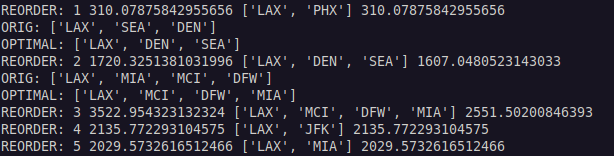
\includegraphics[width=0.9\textwidth, height=0.4\textheight]{images/sorting_output.png}
        \captionof{figure}{Trial Error of the sorting algorithm of three flight routes}
    \end{minipage}
    \vspace{0.5cm} % Add some vertical space between the image and the text
    \begin{minipage}[t]{\textwidth}
        \begin{columns}[t]
            \begin{column}{0.45\textwidth}
            \centering
                \textbf{Overview:}
                \begin{itemize}
                    \item Utilizes Airport IATA Codes as coordinate pair.   
                    \item Sorts the distance using the Haversine formula
                \end{itemize}
            \end{column}
            \begin{column}{0.05\textwidth}
            \end{column}
            \begin{column}{0.5\textwidth}
            \centering
                \textbf{Details:}
                \begin{itemize}
                    \item Explains the importance and impact of sorting distances
                    \item Enhances route efficiency by minimizing travel distance
                \end{itemize}
            \end{column}
        \end{columns}
    \end{minipage}
\end{frame}

%------------------------------------------------
\section{Flight Unsorted}
%------------------------------------------------

\begin{frame}{Visualization of the Sorting Algorithm: Unsorted Flights}
    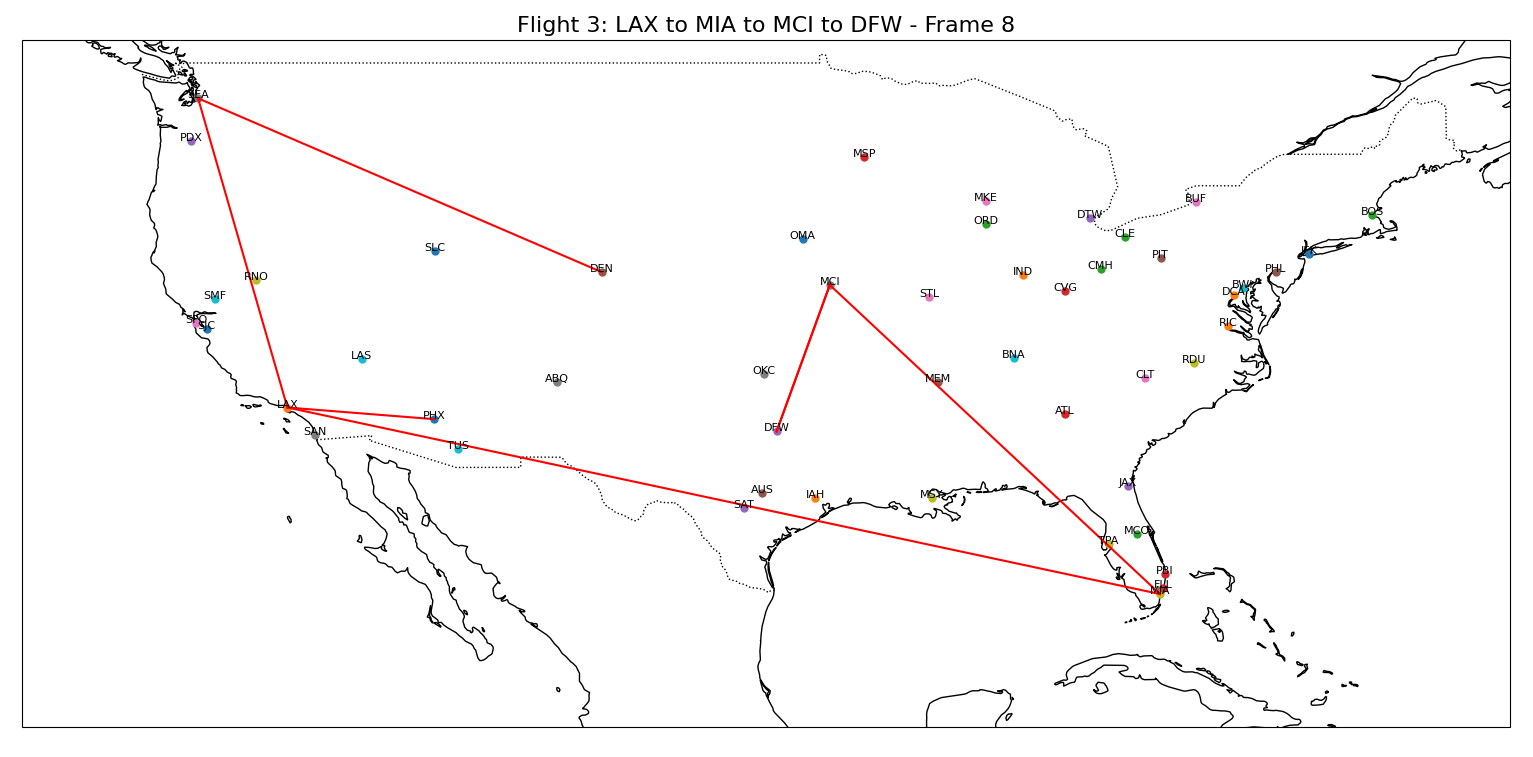
\includegraphics[width=\textwidth]{images/flights_unsort.png}
\end{frame}

%------------------------------------------------
\section{Flight Sorted}
%------------------------------------------------

\begin{frame}{Visualization of Sorting Algorithm: Sorted Flights}
    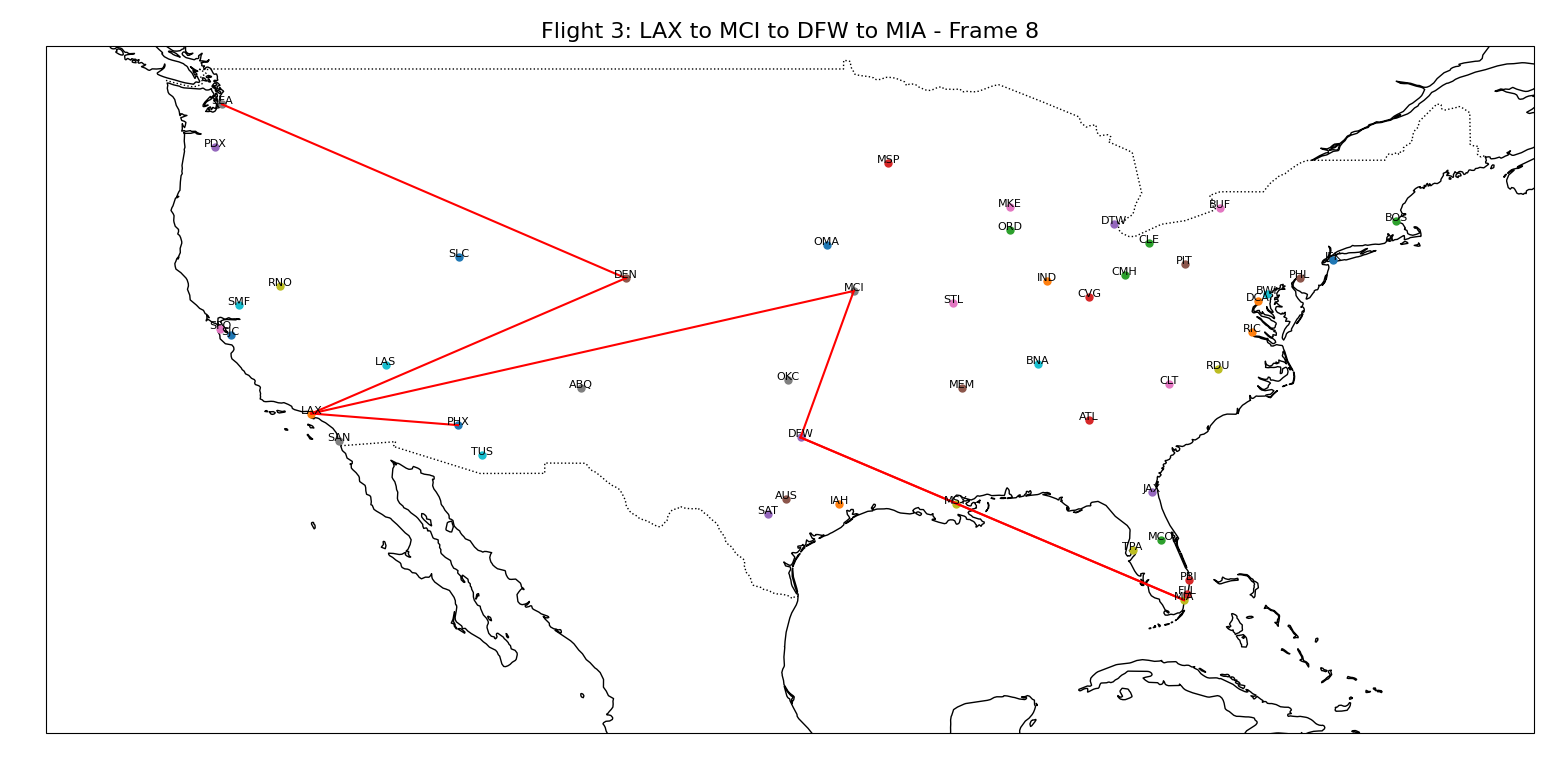
\includegraphics[width=\textwidth]{images/flight_sort.png}
\end{frame}

%------------------------------------------------
\section{Remove and Replace Bad Flights}
%------------------------------------------------

\begin{frame}{Replace Unprofitable Flights}
    \begin{minipage}[t]{\textwidth}
        \centering
        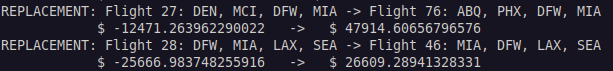
\includegraphics[width=0.9\textwidth, height=0.225\textheight]{images/replace_candidate.png}
        \captionof{figure}{Bad Profitable Flight to Profitable Flight (Net Profits Below Flight Routes).}
    \end{minipage}
    \hfill
    \vspace{0.25cm} % Add vertical space between the image and the text
    \begin{minipage}[t]{\textwidth}
        \begin{columns}[t]
            \begin{column}{0.45\textwidth}
                \centering
                \LARGE\textbf{Overview:}
                \begin{itemize}
                    \large\item Remove Unprofitable Routes
                    \large\item Replace with Nearby Profitable Flights
                \end{itemize}
            \end{column}
            \begin{column}{0.05\textwidth} % Adjust as needed for spacing
            \end{column}
            \begin{column}{0.5\textwidth}
                \centering
                \LARGE\textbf{Details:}
                \begin{itemize}
                    \large\item Matched Closest Profitable Paths
                    \large\item  Adhered to Passenger Capacity Limits
                \end{itemize}
            \end{column}
        \end{columns}
    \end{minipage} 
\end{frame}

%------------------------------------------------
\section{Results and Analysis}
%------------------------------------------------

\begin{frame}{Results} 
    \begin{center}
        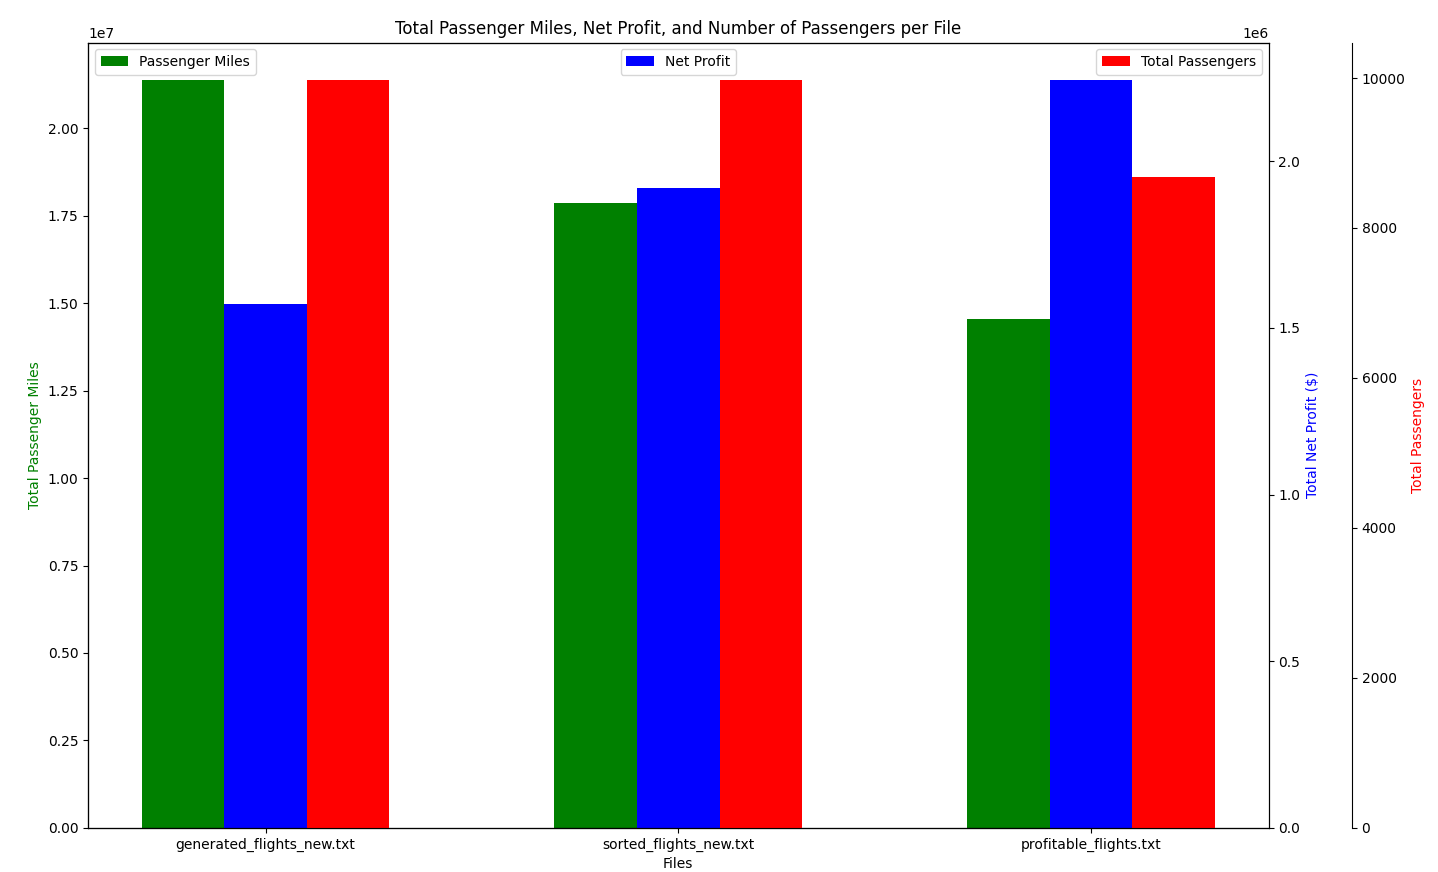
\includegraphics[width=\textwidth, height=0.9\textheight, keepaspectratio]{images/Figure_1.png}
    \end{center} 
\end{frame}

%------------------------------------------------
\section{Future Work}
%------------------------------------------------

\begin{frame}{Future Work}
    \vfill
    \begin{itemize}
        \item Consider passenger boarding and deboarding at intermediate stops.
        \vfill
        \item Incorporate dynamic ticket pricing based on flight distance.
        \vfill
        \item Adapt to real-life flight routes with only an origin and a destination, with no intermediate stops.
        \vfill
        \item Modify Total Passenger Miles also to reflect its contribution to income.
        \vfill
        \item Integrate weather conditions and no-fly zones into the data analysis.
    \end{itemize}
    \vfill
\end{frame}

\end{document}